\documentclass[12pt, openany]{book}

% This is all the packages and settings and so on.
% It is using custom fonts that needs to be installed on the computer. If they are not present, they have to be added manually.
%%%%%%%%%%%%%%%%%%%%%%%%%%%%%%%%%%%%
%%     Include packages          %%
%%%%%%%%%%%%%%%%%%%%%%%%%%%%%%%%%%%%
\usepackage[utf8]{inputenc} % Allows using UTF-8

\usepackage[a4paper, margin=2.56cm]{geometry} % Set-up page and margins

% To insert the pdf frontpage
\usepackage{pdfpages}

% Including some maths utilities
\usepackage{amsmath}
\usepackage{amsfonts}
\usepackage{amsthm}
\usepackage{amssymb}
\DeclareMathOperator*{\argmax}{arg\,max}
\DeclareMathOperator*{\argmin}{arg\,min}


%
% the environments 'definition', 'lemma', 'proposition', 'corollary',
% 'remark', and 'example' are defined in the LLNCS documentclass as well.
%
\newtheorem{definition}{Definition}
\newtheorem{theorem}{Theorem}
\newtheorem{lemma}{Lemma}
\newtheorem{proposition}{Proposition}
\newtheorem{corollary}{Corollary}
\newtheorem{remark}{Remark}
\newtheorem{example}{Example}


% Fancy space between paragraphs
\usepackage{parskip}
\setlength{\parindent}{0em}
\setlength{\parskip}{1em}

% Automatic Month, Year in title
\usepackage{datetime}
\newdateformat{monthyeardate}{
  \monthname[\THEMONTH], \THEYEAR}

% Fancy packages to write pseudocode
\usepackage{algorithm}
\usepackage{algpseudocode}

% Package to import source code and format it
\usepackage{listings}

% Produce more beautiful tables
\usepackage{booktabs}

% Nice hyperlinks inside document
\usepackage[hidelinks]{hyperref}

% Allows enumerating
\usepackage{enumerate}% http://ctan.org/pkg/enumerate

% Required to insert images
\usepackage{graphicx} 

\usepackage[
	citestyle=ieee, 
    bibstyle=ieee,
    style=numeric-comp,
    sorting=nty,
    maxbibnames=99, % Make sure we are printing all authors in the appendix
    backend=biber
]{biblatex}

% Needed to add subcaptions to subfigures
\usepackage{caption}
\usepackage{subcaption}

% Allows using foreach
\usepackage{pgffor}

% Avoids placing floats before section
\usepackage[section]{placeins} 

% Allow to have content in multiple columns
\usepackage{multicol}

% Cool diagrams
\usepackage{tikz}
\usetikzlibrary{positioning,quotes,shapes.geometric,arrows.meta}
\pgfdeclarelayer{nodelayer} 
\pgfdeclarelayer{edgelayer}
\pgfdeclarelayer{embeded}
\pgfdeclarelayer{stages}
\pgfsetlayers{main,nodelayer,edgelayer,stages,embeded}
\tikzstyle{new style 0}=[fill=white, draw=black, shape=circle, align=center]
\tikzstyle{tree_edge}=[-, draw=black]
\tikzstyle{opChan}=[-Stealth, black]
\tikzstyle{daChan}=[-Stealth, red]
\tikzstyle{io}=[trapezium, trapezium angle=67, trapezium stretches body, fill=blue!30, draw=black, thick]
\tikzstyle {filter_gen} = [rectangle, rounded corners, text centered, draw=black, fill=blue!30, thick]
\tikzset{
  invisible/.style={opacity=0},
  visible on/.style={alt={#1{}{invisible}}},
  alt/.code args={<#1>#2#3}{%
    \alt<#1>{\pgfkeysalso{#2}}{\pgfkeysalso{#3}} % \pgfkeysalso doesn't change the path
  },
}
\usepackage{pgf}

% Protect caption to allow \verb
\usepackage{cprotect}
%%%%%%%%%%%%%%%%%%%%%%%%%%%%%%%%%%%%
%%        Usefull macros          %%
%%%%%%%%%%%%%%%%%%%%%%%%%%%%%%%%%%%%

\newcommand{\mst}{\texorpdfstring{$\mathsf{MST}$}{MST}}
\newcommand{\msts}{\texorpdfstring{$\mathsf{MST}s$}{MSTs}}
\newcommand{\mstof}[1]{$\mathsf{MST}_{#1}$}
\newcommand{\dynmst}{\mathsf{Dynamic\_MST}}
\newcommand{\dpm}{\texorpdfstring{$\mathsf{DPA}$}{DPA}}
\newcommand{\DP}{$\mathsf{DP}$}
%\newcommand{\DPmst}{\texorpdfstring{$\mathsf{DP_{MST}}$}{DP\_MST}}
%\newcommand{\DPmstv}[1]{$\mathsf{DP_{MST\_{#1}}}$}

\newcommand{\DPmst}{\texttt{DP\_{Kruskal}}}
\newcommand{\DPmstv}[1]{\texttt{DP\_{Kruskal\_{#1}}}}

\newcommand{\FKruskal}{\texttt{Filter\_{Kruskal}}}
\newcommand{\Kruskal}{\texttt{Kruskal}}

\newcommand{\opinsert}[0]{{\tt insert}}
\newcommand{\opupdate}[0]{{\tt update}}
\newcommand{\opremove}[0]{{\tt remove}}
\newcommand{\opmst}[0]{{\tt mst}}

\newcommand{\Go}{{\tt Go}}
\newcommand{\Golang}{{\tt Golang}}

\newcommand{\AD}[1]{{\color{red} AD: #1} \PackageWarning{teaching}{Comment from AD}}
\newcommand{\DB}[1]{{\color{blue} DB: #1}\PackageWarning{teaching}{Comment from DB}}
\newcommand{\EP}[1]{{\color{magenta} EP: #1}\PackageWarning{teaching}{Comment from EP}}


%%%%%%%%%%%%%%%%%%%%%%%%%%%%%%%%%%%%
%%        Other setups            %%
%%%%%%%%%%%%%%%%%%%%%%%%%%%%%%%%%%%%

\addbibresource{references.bib} % Adds the bibliography

\title{TFM-DanielBenedí}
\author{Daniel Benedí}
\date{\monthyeardate}


% Defining files for bibliography
\addbibresource{references.bib}

% Defining document information
\title{A Concurrent Approach to Fully Dynamic Minimum Spanning Trees}
\author{Daniel Benedí García}

\begin{document}
\setstretch{1.4}

% The front page of the document
\pagenumbering{roman}
\makeatletter
\begin{titlepage}

\vspace*{-4.6\baselineskip}
\hspace*{-0.15\textwidth}
\includegraphics[width=0.2\paperwidth]{setup/img/logo-upc.png}
\par\vspace*{2.5\baselineskip}

\includegraphics[width=0.9\paperwidth]{setup/img/logo-fiblletres-upc-color.png}

~\\

\makebox[0pt][l]{%
\begin{minipage}[b]{0.25\textwidth}
~\\
\end{minipage}
\begin{minipage}{0.65\textwidth}
\begin{center}
{\fontsize{28}{24}\bf\sffamily\@title\\}
\vspace{2cm}
{\fontsize{16}{18}\bf\sffamily \@author}\\
\vspace{2cm}
{\fontsize{16}{18}\sffamily \textbf{Thesis supervisor:} Amalia Duch Brown (Department of Computer Science)}\\
{\fontsize{16}{18}\sffamily \textbf{Thesis co-supervisor:} Edelmira Pasarella Sanchez (Department of Computer Science)}\\
{\fontsize{16}{18}\sffamily \textbf{Degree:} Master Degree in Innovation and Research in Informmatics}\\
{\fontsize{16}{18}\sffamily \textbf{Specialisation:} Advanced Computing}\\
\vspace{1cm}
{\fontsize{16}{18}\sffamily \textbf{Thesis Report}}\\
{\fontsize{16}{18}\sffamily \textbf{Facultat d'Informàtica de Barcelona (FIB)}}\\
{\fontsize{16}{18}\sffamily \textbf{Universitat Politècnica de Catalunya (UPC) - BarcelonaTech}}\\
{\fontsize{16}{18}\sffamily \textbf{XX/YY/2024}}\\
\end{center}
\end{minipage}
}

\end{titlepage}
\makeatother

\newpage
\newpage
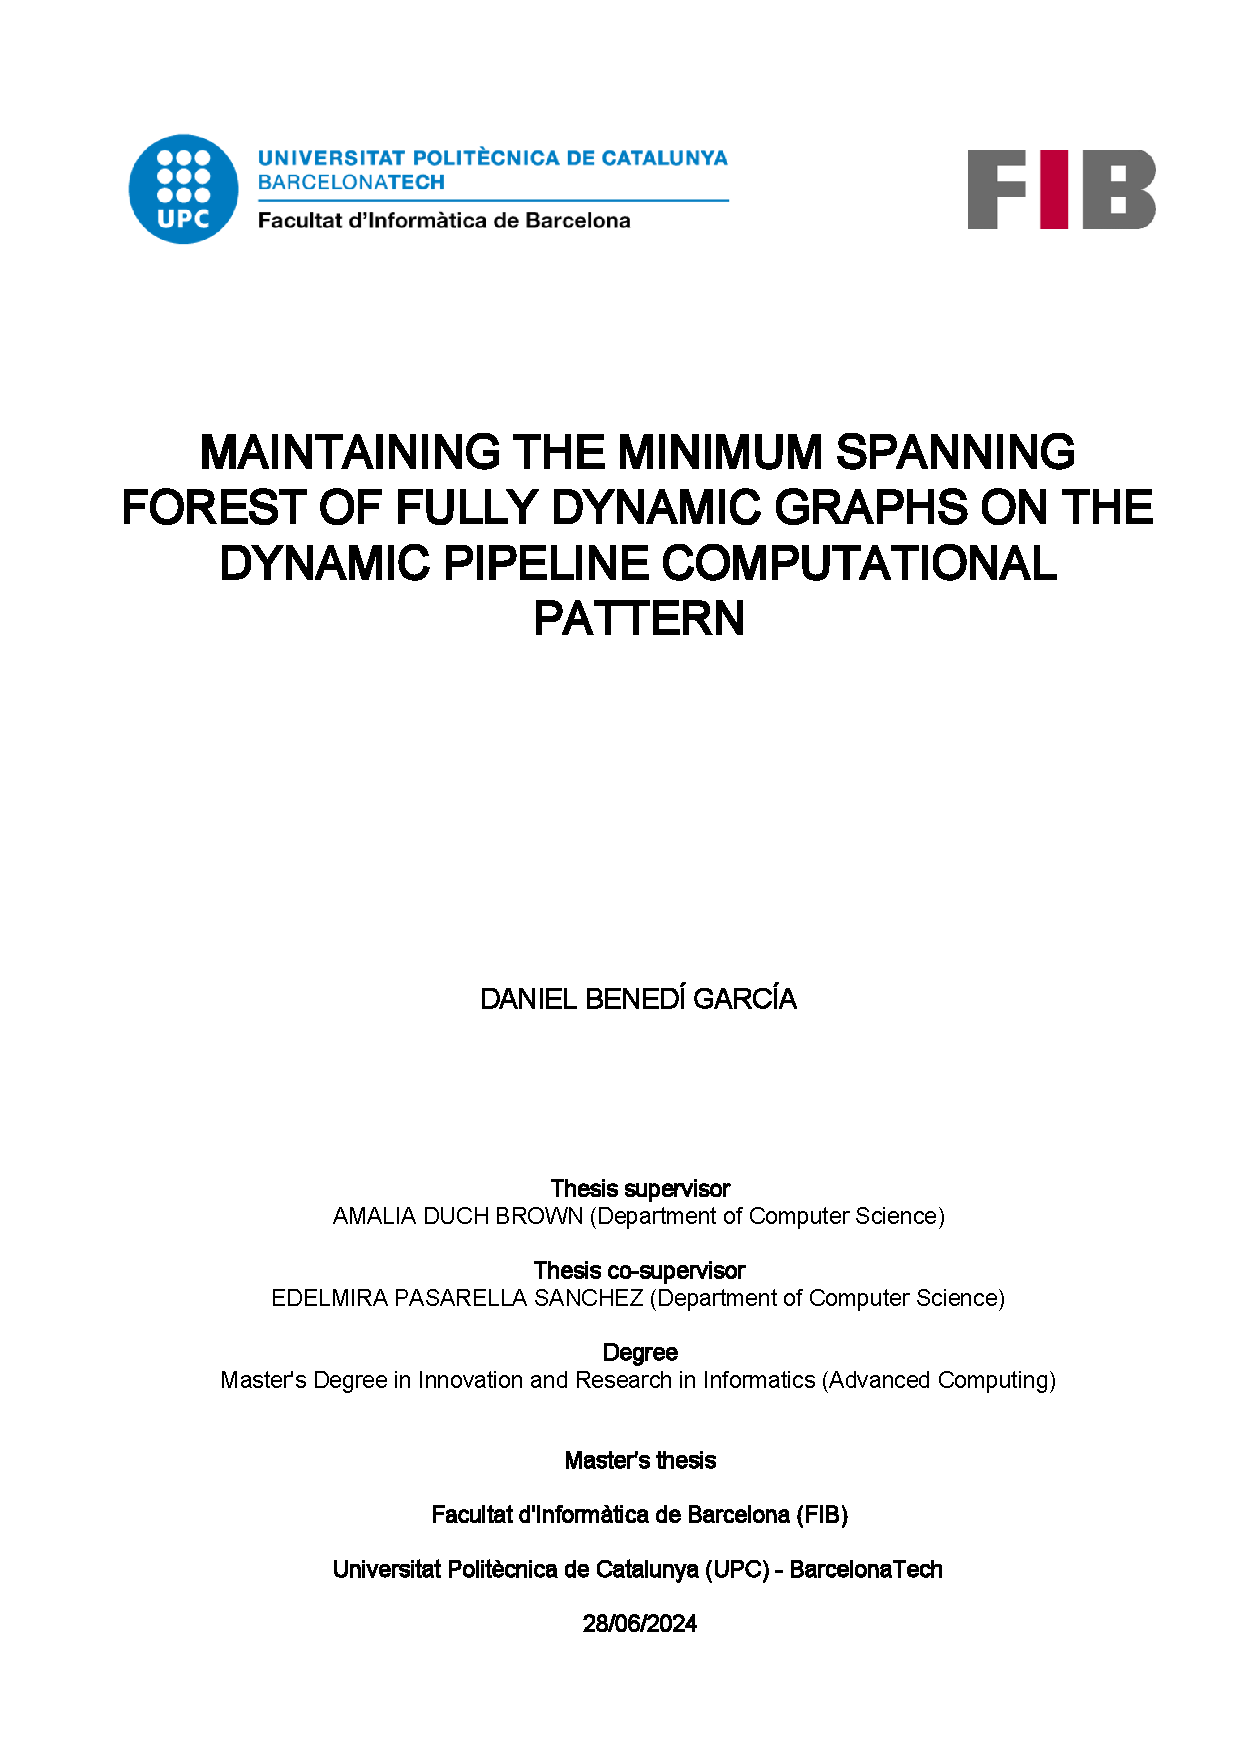
\includepdf{cover.pdf}

\newpage
\thispagestyle{plain}
\begin{flushright}
    
\includegraphics[width=0.8\textwidth]{figures/science.jpg}\\
    I have attempted science - Strange Planet. Nathan W Pyle
\end{flushright}

\newpage

%%%%%%%%%%%%%%%%%%%%%%%%%%%%%%%%%%%%
%%  The English abstract          %%
%%%%%%%%%%%%%%%%%%%%%%%%%%%%%%%%%%%%
\chapter*{Abstract}
%%%%%%%%%%%%%%%%%%%%%%%%%%%%%%%%%%%%
%This work studies the application of the Dynamic Pipeline Approach to parallelize Kruskal's algorithm and thus compute and maintain the Minimum Spanning Tree of dynamic graphs in parallel and distributed settings. To achieve this, we propose to represent the graph through its underlying forest; an adequate representation that enables to store the graph distributed in a dynamic pipeline.
In this work we tackle the problem of using the Dynamic Pipeline Approach to parallelize the Kruskal’s algorithm and thus compute and maintain the Minimum Spanning Tree of dynamic graphs in parallel and distributed settings. To achieve this, we introduce a characterization of  graphs that we call an \emph{underlying forest} of a graph. This characterization gives the basis for representing graphs  in a distributed way along a dynamic pipeline. 

The proposed algorithm, named \DPmst, utilizes a pipeline architecture where the graph is partitioned into trees and distributed across a sequence of stages each handling different aspects of computation. Under this algorithm it possible to keep efficiently graph updates as well as to apply Kruskal's Algorithm at every stage of the pipeline to compute incrementally the minimum spanning tree of the stored graph.

A working implementation was developed to analyze the suitability of \DPmst\ against other algorithms. The programming language \Go\ was chosen because of its concurrency features, as its {\tt goroutines} and  communication channels naturally align with the Dynamic Pipeline Approach.

Several key optimizations were introduced in \DPmst. Some of them regarding the implementation and others the Dynamic Pipeline Approach. Notably, we propose a way to disentangle the message passing from computational tasks which is a general optimization that enhances the entire Dynamic Pipeline Approach framework, not just for \DPmst. These optimizations not only improve program's efficiency but also address and resolve memory management issues within \Go.

Extensive experimental evaluations were conducted to compare \DPmst\ with both sequential and parallel algorithms. Kruskal's algorithm was selected for sequential comparisons, while \FKruskal\ and a message-passing implementation of {\tt Prim}'s algorithm for parallel algorithms. The results demonstrate that \DPmst\ significantly outperforms its counterparts in both single-core and parallel environments, showcasing its superior performance and scalability for handling large and dynamic graphs. 

This work substantiates the effectiveness of the Dynamic Pipeline Approach in addressing complex graph problems and underscores its potential for wider application in parallel computing.


\chapter*{Acknowledgements}
%%%%%%%%%%%%%%%%%%%%%%%%%%%%%%%%%%%%
I would like to express my deepest appreciation to the supervisors of this work, Amalia Duch and Edelmira Pasarella, for their invaluable patience, insightful feedback, and refreshing motivation throughout this journey. Your guidance has been instrumental in the completion of this project.

Additionally, I extend my sincere thanks to the /RDLab-UPC for providing the computational resources necessary for the experimental evaluation. Your support made the technical aspects of this research possible.

I am also grateful to my colleagues and friends from the master program. You provided a warm welcome to this new step in my life, tolerated my moments of stress, and inspired me to dream big. And to my friends from Zaragoza for accompanying me up to this point no matter what happened.

Last but not least, I could not have undertaken this journey without my family and their constant support throughout this research. To my parents, thank you for always supporting me and allowing me to return to my roots; to my sister, for being a beacon of inspiration; and to my significant other, for your constant love and understanding.




\tableofcontents


\pagenumbering{arabic}

``The Future is Big Graphs" states the CACM paper~\cite{sakr2021futureIsBigGraphs} of the same title, where forty-one experts from the data management and large-scale-systems communities settled --after Dagstuhl Seminar 19491 held in Dec. 2019-- their conclusions about the opportunities and challenges of graph processing in the next decade. Beyond the corroboration that graph algorithms should be scalable to deal with the huge amount of data required by nowadays applications, this group of experts claims, among other issues, that, in order to succeed, graph algorithms have to deal with dynamic and streaming aspects of graph processing. This is, coping with updates such as edge insertions, changes, and deletions (dynamicity), as well as indefinitely growth and/or evolution as new data arrive (stream model). Additionally, one of the challenges these experts identified was to define a reference architecture for big graph processing.

Some representative examples are server networks, mobile phone networks, or sensor networks~\cite{Neely2005}, where the devices involved in the network are represented as nodes of a graph and the communications among devices are the weighted edges of the graph, since linking a pair of devices has an associated cost. The resulting resulting graph is fully dynamic as it captures the evolution of the networks along time: new devices can be added to the network, some others might be removed, and the links among them might be modified, involving therefore the insertion and deletion of edges of the graph.

Given an undirected and connected graph with weighted edges, a minimum weight spanning forest, minimum spanning forest, or simply minimum spanning tree (\mst); is a subset of the edges that connects all vertices and has minimum total weight among all such sets. The \mst\ problem is not only of theoretical interest, but also has a wide range of uses, including but not limited to clustering~\cite{AffinityClustering,KHAN20221113}, image segmentation~\cite{Wassenberg2009,LONG2020165308}, and the design of networks~\cite{Li2005}.

To comprehend and forecast the dynamics of evolving networks effectively, it is essential to maintain a minimum weight spanning forest of the dynamic graph. This ensures that the network can be adjusted and reconfigured as new connections are established or existing ones are disconnected. Moreover, in current applications, it is crucial to efficiently compute and maintain a large number of network updates involving potentially a huge number of devices that might be distributed in distant spatial locations~\cite{Tang2009,Tan2010}.

An example of dynamic graphs in which we need to maintain a minimum weight spanning forest can be found in the standard IEEE 802.1Q~\cite{IEEE8021Q}. This standard outlines the support of the Media Access Control (MAC) Service in Bridged Networks, the operational principles of such networks, and the functioning of MAC Bridges and VLAN Bridges, encompassing aspects like management, protocols, and algorithms. In order to provide simple and full connectivity throughout a bridged network comprising arbitrarily interconnected bridges, the Spanning Tree Protocol and some of its variants, such as Rapid Spanning Tree Protocol (RSTP) or the Multiple Spanning Tree Protocol (MSTP), are used in each bridge. The primary purpose of STP is to avoid bridge loops and the broadcast storms they cause. Additionally, Spanning Tree enables a network architecture to incorporate redundant links to ensure system reliability in case a primary link malfunctions.


This work focuses on applying the Dynamic Pipeline Approach (\dpm) \cite{Pasarella2024} to maintain a dynamic graph as well as its \mst\ providing a  parallel Kruskal's algorithm. The study includes the development, optimization, and analysis of the \DPmst\ algorithm. 
Several optimizations are explored from the implementation of the characterization to optimizations of the \dpm\ itself. The performance of \DPmst\ is compared with \FKruskal\ and a message-passing implementation of {\tt Prim}'s algorithm on various graph sizes and densities to assess scalability and efficiency.

%This work focuses on applying the Dynamic Pipeline Approach (\dpm) \cite{Pasarella2024} to parallelize Kruskal's algorithm for computing and maintaining the \mst\ in dynamic graphs using the \Go\ programming language. The study includes the development, optimization, and analysis of the \DPmst\ algorithm, leveraging \Go’s concurrency features like goroutines and channels.

%Key optimizations explored are storing multiple roots per filter, disentangling message passing from MST maintenance, and caching the MST to avoid redundant computations. The performance of \DPmst\ is compared with \FKruskal\ and a message-passing implementation of {\tt Prim}'s algorithm on various graph sizes and densities to assess scalability and efficiency.

The study is limited to specific types of graphs, focusing on random static and real-world dynamic graphs. Experiments are conducted primarily on single-core and multi-core machines, not extending to distributed computing environments. While comparisons with \FKruskal\ and {\tt Prim}'s algorithm are included, not all existing \mst\ algorithms are covered since mostly are theoretical, little implementations are available and it some experimental results show that they do not behave properly in large graphs.

The research does not encompass all possible optimizations or address comprehensive memory management techniques beyond those relevant to \Go\ and \dpm. By defining these boundaries, the study aims to provide a focused investigation into the parallelization of Kruskal's algorithm using \dpm\ within the specified context.


This work comprises five chapters, with this introductory chapter laying the foundation. Chapter~\ref{chap:preliminaries} -Preliminaries- provides an overview of the state of the art, as well as relevant algorithms used throughout the research. Chapter~\ref{chap:dpmst} -\mst\ characterization in the \dpm- explains the main contribution of this project: how the DPA is utilized to solve the \mst problem.Chapter~\ref{chap:experiments} -Experimental Study- describes the experiments conducted, their motivation, the results, and the subsequent analysis. Finally, a conclusion is presented in Chapter~\ref{chap:conclusion}, summarizing the findings and suggesting future research directions.

\include{sections/2-background}
\include{sections/3-method}
\include{sections/4-results}
\include{sections/5-discussion}
\include{sections/6-conclusions}

% \include{content}

\newpage
\addcontentsline{toc}{chapter}{References}
\printbibliography


 \appendix
\chapter{Code for simulate static random graphs in the \DPmst\ \label{appendix:dp_sim:rand}}

\resizebox{\textwidth}{!}{
    \lstinputlisting[language=Python]{code/dp_simulation_random_graph.py}
}

\chapter{Code for simulate real dynamic graphs in the \DPmst\ \label{appendix:dp_sim:real}}

\resizebox{\textwidth}{!}{
    \lstinputlisting[language=Python]{code/dp_simulation_real_graph.py}
}
\include{back-cover}

\end{document}
